
\tikzstyle{Absch} = [rectangle, draw, 
    text centered]
\tikzstyle{keinBeweis} = [rectangle, fill=gray!35, 
    text centered]    

\tikzstyle{BewTeil} = []


\tikzstyle{Box} = [rectangle, draw, text centered, rounded corners]
\tikzstyle{Alg} = [rectangle, draw, fill=gray!50, text centered]
\tikzstyle{Text} = [text centered]
\tikzstyle{Image} = []

\tikzstyle{line} = [draw, -latex']
\tikzstyle{line2} = [draw]


\begin{tikzpicture}[node distance = 5em, auto]

% EINGABE:
\node [Box, text width=20em] (input) {\textbf{Input:} \\ CLR-Instanz $((\ClientSet\cup\FacilitySet,E),c,\phi,d,u)$};
\node [below of=input] (under-input) {};
\node [Image, right of=input, node distance=20em] (input-img) {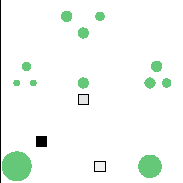
\includegraphics[width=5em]{bilder/instance.pdf}};

% ULF-Instanz:
\node [Box, left of=under-input, text width=12em, node distance=7em] (ULF) {\textbf{ULF-Instanz:} \\ $((\ClientSet\cup\FacilitySet,E),c,\phi,d,u)$};
\node [Text, left of=ULF, text width=12em, node distance=15em] (ULF-lower-bound) {$\leadsto$ Untere Schranke: $\OPT(\CLR) \geq \OPT(\ULF)$};
\node [Alg, below of=ULF, text width=12em] (ULF-solving) {löse approximativ (mit Greedy)};
\node [Image, left of=ULF-solving, node distance=15em] (ULF-img) {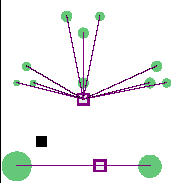
\includegraphics[width=5em]{bilder/ULF.pdf}};

% MST-Instanz:
\node [Box, right of=under-input, text width=12em, node distance=7em] (MST) {\textbf{MST-Instanz:} \\ $((\ClientSet\cup\FacilitySet,E),c,\phi,d,u)$};
\node [Text, right of=MST, text width=12em, node distance=15em] (MST-lower-bound) {$\leadsto$ Untere Schranke: $\OPT(\CLR) \geq \OPT(\MST)$};
\node [Alg, below of=MST, text width=12em] (MST-solving) {löse exakt (mit ???)};
\node [Image, right of=MST-solving, node distance=15em] (MST-img) {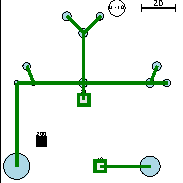
\includegraphics[width=5em]{bilder/MST.pdf}};

% MERGE-Phase:
\node [Alg, below of=under-input, node distance=10em] (merge) {Merge-Phase:};

\node [Text, below of=merge, node distance=2em] (m-facilities) {Eröffne in $\ULF$ oder $\MST$ verwendete Facilities};

\node [Text, below of=m-facilities, node distance=2em] (m-big-clients) {Verbinde Klienten $v$ mit $d(v)\geq u$ mit nächstliegender offener Fabrik};
\node [Image, right of=m-big-clients, node distance=25em] () {
	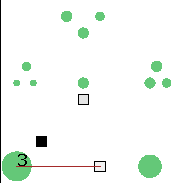
\includegraphics[width=5em]{bilder/largeDemand1.pdf}
	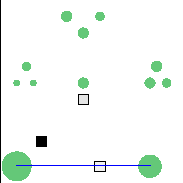
\includegraphics[width=5em]{bilder/largeDemand2.pdf}
};

\node [Text, below of=m-big-clients, node distance=2em] (m-small-clients) {Für jede durch die $\MST$-Lsg eröffnete Farbik $f$ tue...};

\node [Box, below of=m-small-clients, node distance=10em] (m-relieve) {
		\begin{minipage}{20em}
			\begin{algorithmic}
			\While{$D_f > 0$}
			\State Finde $v \in S_f$ mit $D_v > u$ und f.a. Kinder $w$ von $v$: $D_w \leq u$
			\State Zerlege $S_v$ in Teilbäume ...
			\EndWhile
			\end{algorithmic}
		\end{minipage}
	};
\node [Image, right of=m-relieve, node distance=25em] () {
		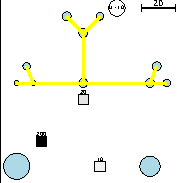
\includegraphics[width=5em]{bilder/relieveTour1.pdf}
		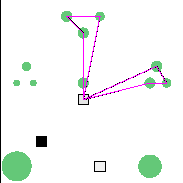
\includegraphics[width=5em]{bilder/relieveTour2.pdf}
		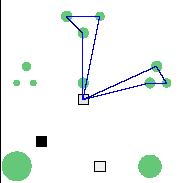
\includegraphics[width=5em]{bilder/relieveTour3.pdf}
	};

\node [Text, below of=m-relieve, node distance=5em] (m-remaining) {Mache rest...};
\node [Image, right of=m-remaining, node distance=25em] () {
	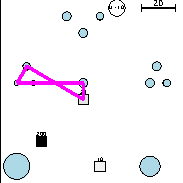
\includegraphics[width=5em]{bilder/remainingTour1.pdf}
	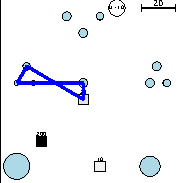
\includegraphics[width=5em]{bilder/remainingTour2.pdf}
};

% AUSGABE:
\node [Box, below of=m-remaining, node distance=5em] (output) {Lösung};
\node [Image, right of=output, node distance=20em] (outpu-img) {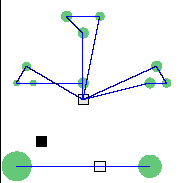
\includegraphics[width=5em]{bilder/output.pdf}};


% PATHS:

\path [line] (input.south) -- (ULF.north);    
\path [line] (input.south) -- (MST.north); 

\path [line] (ULF-solving.south) -- (merge.north);
\path [line] (MST-solving.south) -- (merge.north);

\path [line] (m-remaining.south) -- (output.north);

\end{tikzpicture}
